\documentclass[12pt,a4paper]{article}
\usepackage[utf8]{inputenc}
\usepackage{polski}
\usepackage{amsmath}
\usepackage{amssymb}
\usepackage{amsfonts}
\usepackage{geometry}
\usepackage{graphicx}
\usepackage{listings}
\usepackage{xcolor}

\geometry{top=2.5cm, bottom=2.5cm, left=2.5cm, right=2.5cm}

% Konfiguracja wyglądu kodu źródłowego (zgodnie z report.pdf)
\definecolor{commentgreen}{rgb}{0,0.6,0}
\definecolor{gray}{rgb}{0.5,0.5,0.5}
\definecolor{keywordblue}{rgb}{0.1,0.1,0.8}

\lstset{
    backgroundcolor=\color{white},
    commentstyle=\color{commentgreen},
    keywordstyle=\color{keywordblue},
    numberstyle=\tiny\color{gray},
    stringstyle=\color{purple},
    basicstyle=\ttfamily\footnotesize,
    breakatwhitespace=false,         
    breaklines=true,                 
    captionpos=b,                    
    keepspaces=true,                 
    numbers=left,                    
    numbersep=5pt,                  
    showspaces=false,                
    showstringspaces=false,
    showtabs=false,                  
    tabsize=4,
    language=Python
}

\title{Wybrane zagadnienia Algebry 2026\\{\Large Sprawozdanie 2.}}
\author{Sara Żyndul\\279686}

\begin{document}

\maketitle

\section{Laboratorium 4: Wielomiany wielu zmiennych i bazy Gröbnera}

\subsection{Ad a) Pierścienie wielomianów wielu zmiennych i różnice w implementacji}

Wielomiany wielu zmiennych w pierścieniu $\mathbb{R}[x_1, \dots, x_n]$ zostały zaimplementowane w oparciu o strukturę słownikową (tzw. reprezentację rzadką). Każdy wielomian reprezentowany jest jako obiekt, w którym:
\begin{itemize}
    \item \textbf{Klucz słownika} (dictionary key) stanowi wektor potęg poszczególnych zmiennych zapisany w postaci niemutowalnej krotki (\texttt{tuple}). Na przykład w pierścieniu $\mathbb{R}[x, y, z]$ krotka \texttt{(2, 7, 0)} jednoznacznie odpowiada jednomianowi $x^2y^7$.
    \item \textbf{Wartość słownika} (dictionary value) odpowiada niezerowemu współczynnikowi rzeczywistemu (użytemu jako klasa \texttt{Fraction}) stojącemu przy danym jednomianie.
\end{itemize}

\noindent \textbf{Różnice w implementacji względem wielomianów jednej zmiennej:}
\begin{enumerate}
    \item \textbf{Struktura danych:} W przypadku jednej zmiennej jednomiany można wydajnie reprezentować za pomocą zwykłej listy, gdzie indeks elementu bezpośrednio wyznacza potęgę zmiennej (reprezentacja gęsta). Dla wielu zmiennych liczba potencjalnych kombinacji wykładników rośnie wykładniczo, co przy reprezentacji gęstej prowadziłoby do wybuchu pamięciowego. Reprezentacja rzadka (słownikowa) przechowuje wyłącznie niezerowe składniki.
    \item \textbf{Brak naturalnego porządku:} Wielomiany jednej zmiennej posiadają naturalny, jednoznaczny i liniowy porządek jednomianów wyznaczany przez ich stopień ($x^0 < x^1 < x^2 < \dots$). Wyznaczenie wyrazu wiodącego (\textit{Leading Term}, LT) jest tam trywialne. W przypadku wielu zmiennych nie istnieje jeden naturalny porządek (porównanie jednomianów $x^2$ oraz $y^3$ zależy wyłącznie od przyjętej konwencji). Z tego powodu klasa musi jawnie przyjmować ciąg zmiennych (\texttt{vars}) oraz kryterium porządku (np. \texttt{order\_vars}), na podstawie którego dynamicznie mapuje krotki wykładników za pomocą dedykowanych funkcji klucza (\texttt{lex\_key}).
\end{enumerate}

\subsection{Ad b) Implementacja operacji redukcji, syzygium oraz algorytmu Buchbergera}

W celu generowania baz Gröbnera zaimplementowano trzy kluczowe operacje algebraiczne:
\begin{itemize}
    \item \textbf{\texttt{PolynomialReduce(f, G)}}: Realizuje zachłanny algorytm dzielenia wielomianu $f$ przez ciąg wielomianów $\mathcal{G} = (g_1, \dots, g_k)$. W każdej iteracji algorytm sprawdza, czy wyraz wiodący aktualnego wielomianu $p$ jest podzielny przez wyraz wiodący któregokolwiek z dzielników $g_i$. Jeśli tak, dokonuje redukcji; w przeciwnym wypadku przenosi wyraz wiodący do reszty $r$.
    \item \textbf{\texttt{Syzygy(f, g)}}: Wyznacza S-wielomian (syzygium) dla pary wielomianów $f$ i $g$. Operacja ta polega na znalezieniu najmniejszej wspólnej wielokrotności (\textit{LCM}) ich wykładników wiodących, a następnie ich wzajemnym skróceniu (eliminacji najwyższych składników):
    \begin{equation}
        S(f,g) = \frac{x^\gamma}{LT(f)}\cdot f - \frac{x^\gamma}{LT(g)}\cdot g, \quad \text{gdzie } x^\gamma = \text{lcm}(LM(f), LM(g))
    \end{equation}
    \item \textbf{\texttt{Buchberger(G\_init)}}: Konstruuje bazę Gröbnera poprzez sukcesywne badanie redukcji S-wielomianów dla wszystkich par wielomianów znajdujących się w bazie. Jeśli reszta z redukcji $S(g_i, g_j)$ przez aktualną bazę jest niezerowa, jest ona dopisywana do zbioru generatorów. Proces kończy się, gdy wszystkie pary redukują się do zera. Na koniec baza zostaje zminimalizowana i w pełni zredukowana.
\end{itemize}


\noindent Poniżej przedstawiono kompletną implementację tych algorytmów w języku Python:

\begin{lstlisting}[caption={Kody źródłowe funkcji algorytmu Buchbergera}]
def polynomial_reduce(f, G, order_vars=None):
    if order_vars is None:
        order_vars = f.vars
    vars_list = f.vars
    
    r = Polynomial({}, vars_list)
    p = Polynomial(f.terms, vars_list)
    
    while not p.is_zero():
        lt_p_exps, lt_p_coeff = p.leading_term(order_vars)
        reduced = False
        for g in G:
            if g.is_zero():
                continue
            lt_g_exps, lt_g_coeff = g.leading_term(order_vars)
            div = divide_monomials(lt_p_exps, lt_g_exps)
            if div is not None:
                # p = p - (lt_p / lt_g) * g
                mono_dict = {div: lt_p_coeff / lt_g_coeff}
                monomial_poly = Polynomial(mono_dict, vars_list)
                p = p - monomial_poly * g
                reduced = True
                break
        if not reduced:
            # lt_p nie jest redukowalny przez zadne g_i -> trafia do reszty
            r = r + Polynomial({lt_p_exps: lt_p_coeff}, vars_list)
            p = p - Polynomial({lt_p_exps: lt_p_coeff}, vars_list)
    return r

def syzygy(f, g, order_vars=None):
    if f.is_zero() or g.is_zero():
        return Polynomial({}, f.vars)
    lt_f_exp, lt_f_coeff = f.leading_term(order_vars)
    lt_g_exp, lt_g_coeff = g.leading_term(order_vars)
    
    lcm_exp = lcm_monomials(lt_f_exp, lt_g_exp)
    
    div_f = divide_monomials(lcm_exp, lt_f_exp)
    div_g = divide_monomials(lcm_exp, lt_g_exp)
    
    S_f = Polynomial({div_f: Fraction(1, lt_f_coeff)}, f.vars) * f
    S_g = Polynomial({div_g: Fraction(1, lt_g_coeff)}, g.vars) * g
    return S_f - S_g

def buchberger(G_init, order_vars=None):
    G = [g for g in G_init if not g.is_zero()]
    pairs = [(G[i], G[j]) for i in range(len(G)) for j in range(i+1, len(G))]
    
    while pairs:
        g1, g2 = pairs.pop(0)
        S = syzygy(g1, g2, order_vars)
        rem = polynomial_reduce(S, G, order_vars)
        if not rem.is_zero():
            for g in G:
                pairs.append((g, rem))
            G.append(rem)
            
    # Minimalizacja i redukcja bazy Groebnera
    cleaned_G = []
    for g in G:
        lt_exp, lt_coeff = g.leading_term(order_vars)
        zero_tuple = (0,) * len(g.vars)
        cleaned_G.append(g * Polynomial({zero_tuple: Fraction(1, lt_coeff)}, g.vars))
        
    reduced_G = []
    for i in range(len(cleaned_G)):
        other_G = cleaned_G[:i] + cleaned_G[i+1:]
        rem = polynomial_reduce(cleaned_G[i], other_G, order_vars)
        if not rem.is_zero():
            lt_exp, lt_coeff = rem.leading_term(order_vars)
            zero_tuple = (0,) * len(rem.vars)
            rem = rem * Polynomial({zero_tuple: Fraction(1, lt_coeff)}, rem.vars)
            if rem.terms not in [r.terms for r in reduced_G]:
                reduced_G.append(rem)
    return reduced_G
\end{lstlisting}





\subsection{Ad c) Analiza układu stożka i płaszczyzn (eliminacja zmiennych)}

Rozważamy układ równań składający się ze stożka $x^2 + y^2 = z^2$ oraz płaszczyzn $f(x,y,z) = 0$. W celu eliminacji zmiennej $z$ z układu i wyznaczenia ideału głównego $\mathcal{I}_f$ w pierścieniu $\mathbb{R}[x,y]$, wygenerowano bazy Gröbnera przy użyciu porządku leksykograficznego $z > x > y$. 

Wielomian niezawierający zmiennej $z$ stanowi poszukiwany generator ideału. Poniżej przedstawiono wyniki działania zaimplementowanego algorytmu Buchbergera dla stałych z numeru indeksu ($a=2, c=9, d=6, e=8, f=6$) wraz z rzutami geometrycznymi otrzymanych rozmaitości $V(\mathcal{I}_f)$ na płaszczyznę XY (tzw. krzywych stożkowych).

\begin{itemize}
    \item \textbf{Przypadek 1:} $f(x,y,z) = (c+1)z = 10z$ \vspace{0.5em}\\
    \begin{minipage}[c]{0.55\textwidth}
        \begin{itemize}
            \item \textbf{Ideał główny:} $\mathcal{I}_{f_1} = \langle x^2 + y^2 \rangle$
            \item \textbf{Rozmaitość:} Pojedynczy punkt $(0,0)$.
            \item \textbf{Uzasadnienie geometryczne:} Płaszczyzna $z=0$ przecina stożek dokładnie w jego wierzchołku, nie obejmując żadnych innych punktów.
        \end{itemize}
    \end{minipage}\hfill
    \begin{minipage}[c]{0.3\textwidth}
        \centering
        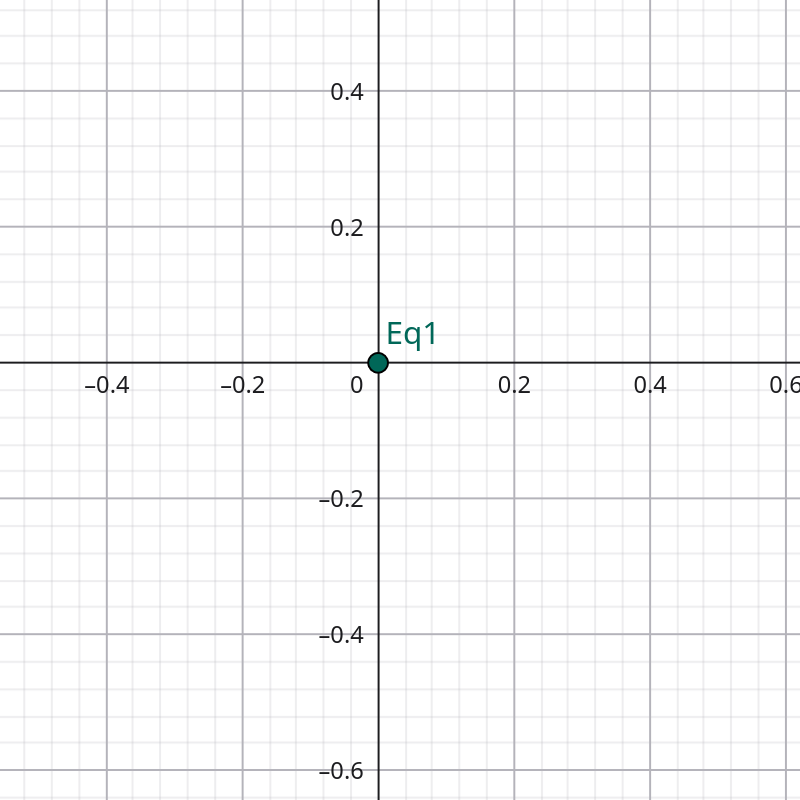
\includegraphics[width=\linewidth]{plots/c1.png}
    \end{minipage}
    \vspace{1em}

    \item \textbf{Przypadek 2:} $f(x,y,z) = z + d + 1 = z + 7$ \vspace{0.5em}\\
    \begin{minipage}[c]{0.55\textwidth}
        \begin{itemize}
            \item \textbf{Ideał główny:} $\mathcal{I}_{f_2} = \langle x^2 + y^2 - 49 \rangle$
            \item \textbf{Rozmaitość:} Okrąg o promieniu $R=7$.
            \item \textbf{Uzasadnienie geometryczne:} Płaszczyzna $z=-7$ jest prostopadła do pionowej osi stożka. Poziome cięcie stożka obrotowego zawsze generuje okrąg.
        \end{itemize}
    \end{minipage}\hfill
    \begin{minipage}[c]{0.3\textwidth}
        \centering
        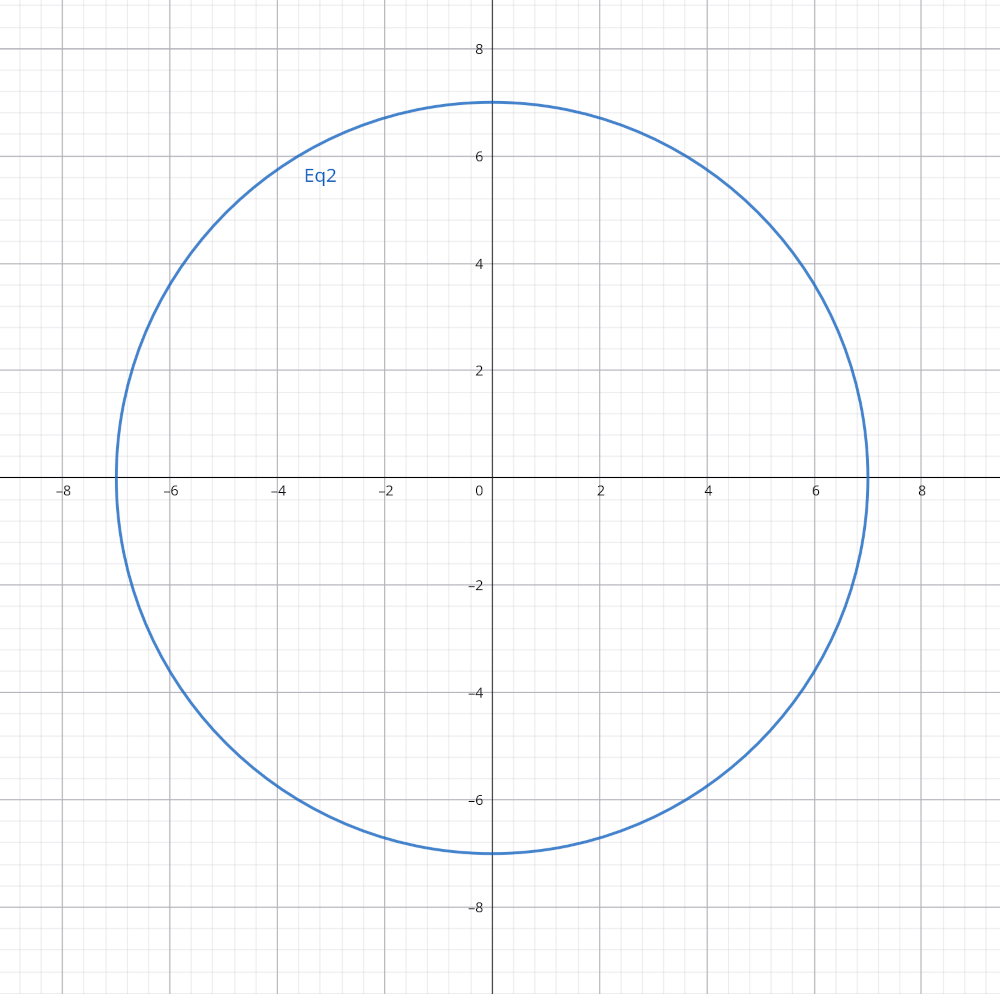
\includegraphics[width=\linewidth]{plots/c2.png}
    \end{minipage}
    \vspace{1em}

    \item \textbf{Przypadek 3:} $f(x,y,z) = x + z - e - 1 = x + z - 9$ \vspace{0.5em}\\
    \begin{minipage}[c]{0.55\textwidth}
        \begin{itemize}
            \item \textbf{Ideał główny:} $\mathcal{I}_{f_3} = \langle x + \frac{1}{18}y^2 - \frac{9}{2} \rangle$
            \item \textbf{Rozmaitość:} Parabola.
            \item \textbf{Uzasadnienie geometryczne:} Płaszczyzna tnąca jest nachylona do osi stożka pod tym samym kątem, co jego boczna tworząca. Skutkuje to powstaniem otwartej krzywej parabolicznej.
        \end{itemize}
    \end{minipage}\hfill
    \begin{minipage}[c]{0.3\textwidth}
        \centering
        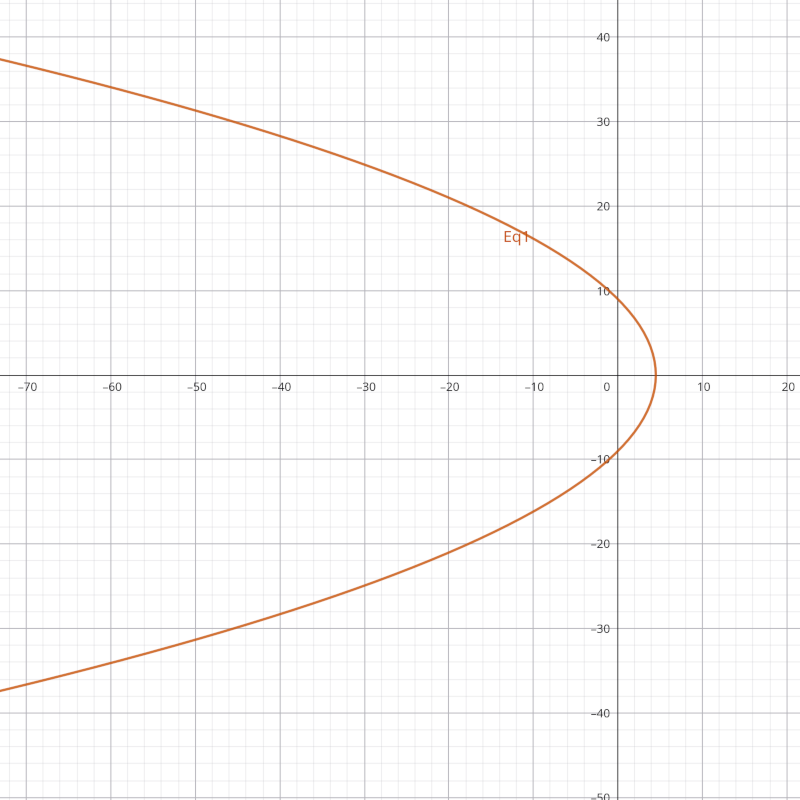
\includegraphics[width=\linewidth]{plots/c3.png}
    \end{minipage}
    \vspace{1em}

    \item \textbf{Przypadek 4:} $f(x,y,z) = x + y + z + f + 1 = x + y + z + 7$ \vspace{0.5em}\\
    \begin{minipage}[c]{0.55\textwidth}
        \begin{itemize}
            \item \textbf{Ideał główny:} $\mathcal{I}_{f_4} = \langle xy + 7x + 7y + \frac{49}{2} \rangle$
            \item \textbf{Rozmaitość:} Hiperbola.
            \item \textbf{Uzasadnienie geometryczne:} Stromo nachylona płaszczyzna przecina obie połacie stożka (górną i dolną), tworząc krzywą składającą się z dwóch oddzielnych gałęzi.
        \end{itemize}
    \end{minipage}\hfill
    \begin{minipage}[c]{0.3\textwidth}
        \centering
        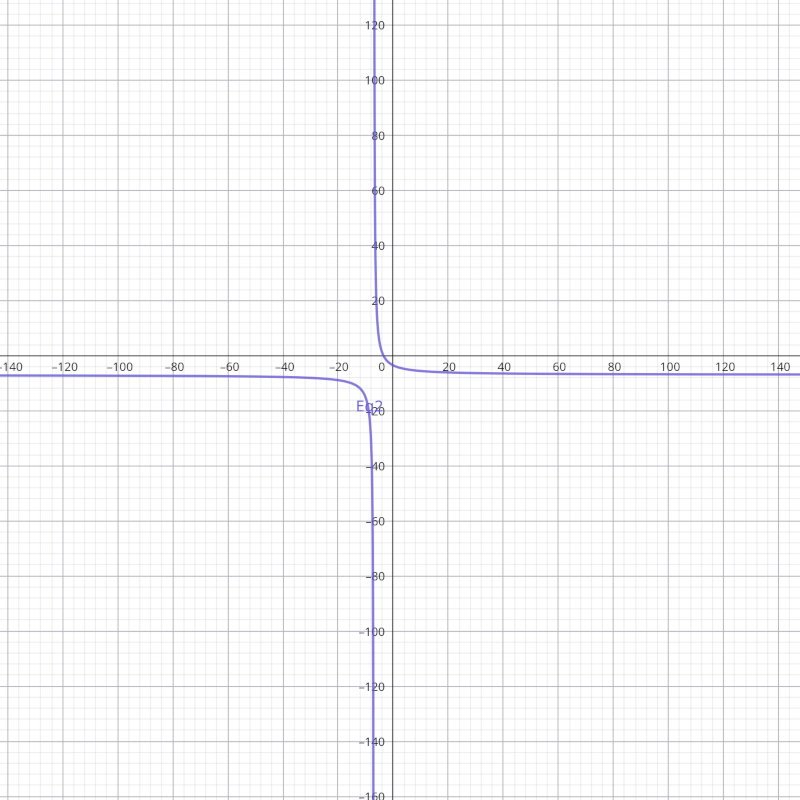
\includegraphics[width=\linewidth]{plots/c4.png}
    \end{minipage}
    \vspace{1em}

    \item \textbf{Przypadek 5:} $f(x,y,z) = \frac{y}{a} + z + 1 = \frac{1}{2}y + z + 1$ \vspace{0.5em}\\
    \begin{minipage}[c]{0.55\textwidth}
        \begin{itemize}
            \item \textbf{Ideał główny:} $\mathcal{I}_{f_5} = \langle x^2 + \frac{3}{4}y^2 - y - 1 \rangle$
            \item \textbf{Rozmaitość:} Elipsa.
            \item \textbf{Uzasadnienie geometryczne:} Płaszczyzna przecina stożek na wskroś, obejmując tylko jedną połać, ale pod kątem mniejszym niż nachylenie tworzącej. Generuje to krzywą zamkniętą. Dodatnie i różne współczynniki przy $x^2$ i $y^2$ potwierdzają kształt elipsy.
        \end{itemize}
    \end{minipage}\hfill
    \begin{minipage}[c]{0.3\textwidth}
        \centering
        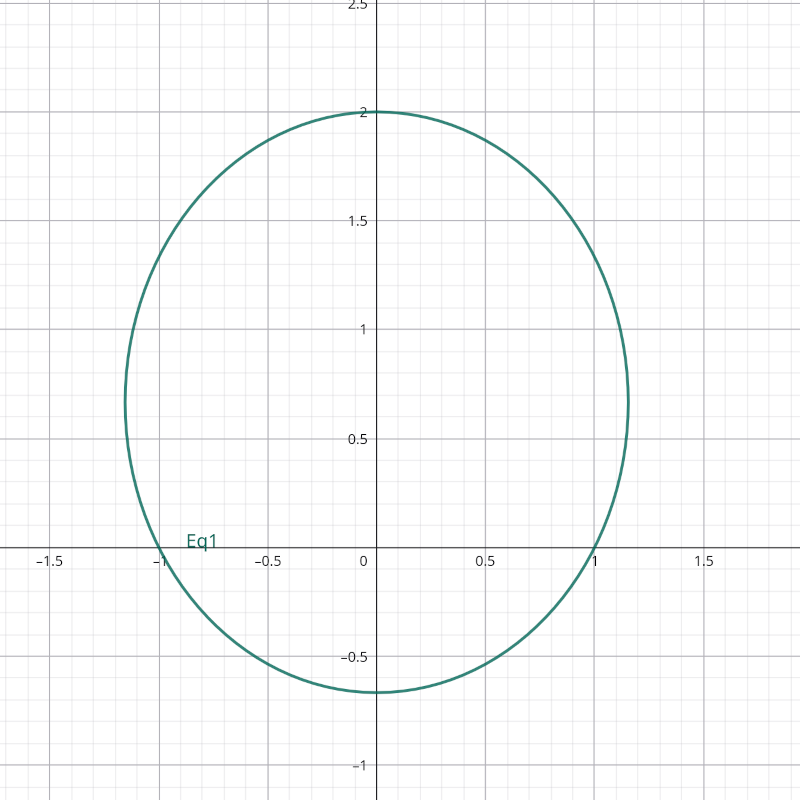
\includegraphics[width=\linewidth]{plots/c5.png}
    \end{minipage}
\end{itemize}




\subsection{Ad d) Eliminacja zmiennej $x$ oraz analiza przekroju kardioidalnego}

W tym punkcie poddano analizie układ równań wyższego stopnia, w którym pierwsze równanie definiuje powierzchnię stożka kardioidalnego, a drugie płaszczyznę tnącą:
\begin{equation}
\begin{cases} 
(x^2 + y^2 - ax)^2 = z^2(x^2 + y^2) \\ 
x + 2y + 3z = 0 
\end{cases}
\end{equation}

Dla wartości parametru $a = 2$ wyznaczono bazę Gröbnera przy porządku leksykograficznym $x > y > z$, co pozwoliło na całkowite wyeliminowanie zmiennej $x$ i uzyskanie generatora ideału w pierścieniu $\mathbb{R}[y,z]$.

\begin{itemize}
    \item \textbf{Wykres 1 (Rzut rozwiązania układu na płaszczyznę YZ):} \vspace{0.5em}\\
    \begin{minipage}[c]{0.55\textwidth}
        Wyselekcionowany z bazy wielomian eliminacji zmiennej $x$ przyjmuje postać:
        \[ y^4 + \frac{24}{5}y^3z + \frac{8}{5}y^3 + \frac{229}{25}y^2z^2 + \frac{156}{25}y^2z + \frac{16}{25}y^2 \]
        \[ + \frac{204}{25}yz^3 + \frac{216}{25}yz^2 + \frac{48}{25}yz + \frac{72}{25}z^4 + \frac{108}{25}z^3 + \frac{36}{25}z^2 = 0 \]
        Generuje on płaską krzywą algebraiczną stopnia 4 (kwartykę), przedstawiającą geometryczny rzut linii przecięcia płaszczyzny z powierzchnią na płaszczyznę współrzędnych $yz$.
    \end{minipage}\hfill
    \begin{minipage}[c]{0.4\textwidth}
        \centering
        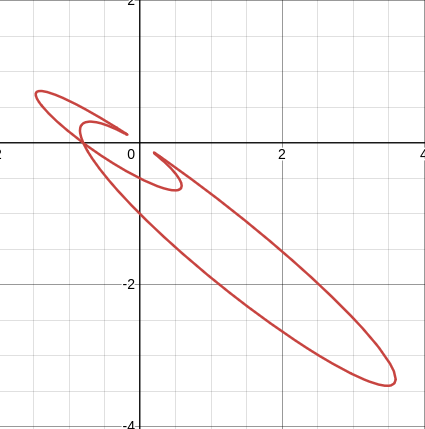
\includegraphics[width=\linewidth]{plots/d1.png}
    \end{minipage}
    \vspace{1.5em}

    \item \textbf{Wykres 2 (Przekrój powierzchni dla $z = a = 2$):} \vspace{0.5em}\\
    \begin{minipage}[c]{0.55\textwidth}
        Rozważając wyłącznie pierwsze równanie wyjściowe dla stałej wysokości $z = 2$, otrzymujemy relację:
        \[ (x^2 + y^2 - 2x)^2 = 4(x^2 + y^2) \]
        Przejście do układu biegunowego ($x = r\cos\theta$, $y = r\sin\theta$) pozwala uprościć to wyrażenie do postaci:
        \[ (r^2 - 2r\cos\theta)^2 = 4r^2 \implies r = 2(1 + \cos\theta) \]
        Krzywa ta to klasyczna \textbf{kardioida}. Dowodzi to, że badana powierzchnia trójwymiarowa jest strukturą, której poziome przekroje są skalowanymi i przesuniętymi kardioidami.
    \end{minipage}\hfill
    \begin{minipage}[c]{0.4\textwidth}
        \centering
        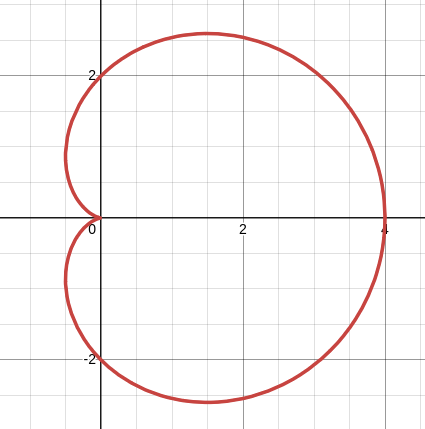
\includegraphics[width=\linewidth]{plots/d2.png}
    \end{minipage}
\end{itemize}





\subsection{Ad e) Wyznaczenie równania kartezjańskiego i analiza otrzymanej krzywej}

Przedmiotem analizy jest krzywa zdefiniowana w układzie biegunowym równaniem podanym w zadaniu:
\begin{equation}
r = b\left(4\cos(\theta) + \frac{1}{\cos(\theta)}\right)
\end{equation}

Dla przydzielonej wartości parametru $b = 7$ równanie to przybiera postać $r = 28\cos(\theta) + \frac{7}{\cos(\theta)}$. Wykorzystując związki transformacji biegunowej ($x = r\cos(\theta)$, $y = r\sin(\theta)$, $r^2 = x^2 + y^2$) oraz zaimplementowany algorytm baz Gröbnera do eliminacji zmiennych, wyznaczono jawne równanie algebraiczne w układzie kartezjańskim.

\vspace{1em}
\begin{minipage}[c]{0.55\textwidth}
    \begin{itemize}
        \item \textbf{Postać wielomianowa:} 
        \[ x^3 + xy^2 - 35x^2 - 7y^2 = 0 \]
        \item \textbf{Własności geometryczne:} Po przekształceniu równania do postaci $y^2 = \frac{x^2(35-x)}{x-7}$ łatwo zauważyć, że ciągła gałąź krzywej istnieje wyłącznie dla domeny $x \in (7, 35]$. Z lewej strony ogranicza ją asymptota pionowa $x = 7$, a z prawej wierzchołek w punkcie $(35, 0)$.
        \item \textbf{Punkt izolowany:} Z matematycznego punktu widzenia, równanie jest spełnione również dla punktu $(0,0)$. Jest to jednak punkt izolowany (odosobniony), którego standardowe narzędzia graficzne nie renderują, stąd krzywa wizualnie omija początek układu współrzędnych.
        \item \textbf{Uwaga do trysektrysy:} Klasyczna trysektrysa Maclaurina (służąca historycznie do geometrycznego podziału kąta na trzy części) posiada w swoim równaniu biegunowym znak minus. Zastosowanie znaku plus (zgodnie z treścią zadania) spowodowało "otwarcie" charakterystycznej pętli i powstanie krzywej o zbadanych wyżej właściwościach.
    \end{itemize}
\end{minipage}\hfill
\begin{minipage}[c]{0.4\textwidth}
    \centering
    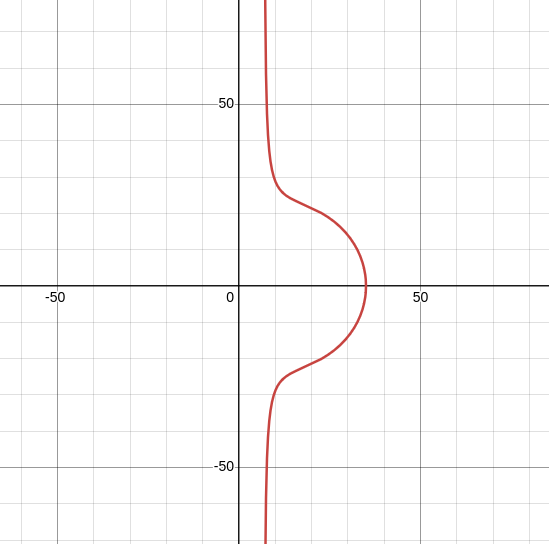
\includegraphics[width=\linewidth]{plots/e.png}
\end{minipage}

\end{document}